\section{Ejercicio 3}

\begin{table}[H]
	\begin{center}
	\scalebox{0.8}{
		\begin{tabular}{c|c|c}
		Estado & $Q_1$                  & $Q_0$ \\ \hline
		A      & \multicolumn{1}{c|}{0} & 0     \\
		B      & \multicolumn{1}{c|}{0} & 1     \\
		C      & \multicolumn{1}{c|}{1} & 0     \\
		\end{tabular}
	}
	\caption{Estados utilizados}
	\end{center}
	\label{Estados_Ej3}
\end{table}

\begin{table}[H]
\begin{center}
\scalebox{0.8}{
\begin{tabular}{c|cc|c}
\multirow{2}{*}{Estado Actual} & \multicolumn{2}{c|}{Entrada} & Salida \\
                               & X=0                    & X=1 & S      \\ \hline
A                              & \multicolumn{1}{c|}{A} & B   & 0      \\
B                              & \multicolumn{1}{c|}{A} & C   & 1      \\
C                              & \multicolumn{1}{c|}{A} & C   & 0     
\end{tabular}
}
\label{Tabla_de_transiciones_Ej3}
\caption{Tabla de transiciones}
\end{center}
\end{table}

 \begin{figure}[H]
\begin{center}
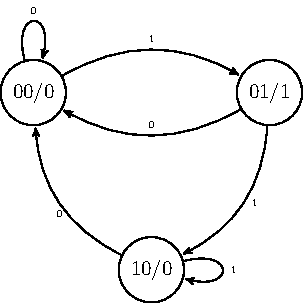
\includegraphics[scale=0.75]{Ejercicio3/Diagramas/TransicionesEj3}
\caption{Diagrama de estados}
\end{center}
\label{Diagrama_de_estados_Ej3}
\end{figure}

%Mapas de Karnaugh 
\subsection{Implementación}
\begin{center}
	\hspace*{\fill}
   \begin{tikzpicture}[x=8mm,y=8mm]
    \K[x bits = 2, y bits = 1, label={$D_1$},
       variable names = {$Q_0$,$X$,$Q_1$,}]
    { 
      000,0,    
      001,0,   
      010,0,   
      011,1,       
      100,0, 
      101,X,
      110,1,
 	  111,X,

    }
    \newcommand*{\myKG}[4][0.1]{\KG[x bits = 2,y bits = 1,group opacity = #1,
                  #2]{#3}{#4}}
    \myKG     {group color = red,  group distance=0.35}{011}{111}
    \myKG     {group color = pink,  group distance=0.35}{111}{110}



    %=====================================================================
    % in picture comments
    %=====================================================================

    \path (1,-1.5) node[anchor = north, align = left] (eq1){%
    $D_1 = 
       \ul{red}{${Q_0X}\,$}
       +\ul{pink}{${Q_1X}\,$}  
    $};
    
  \end{tikzpicture}
	\hspace{2mm}
   \begin{tikzpicture}[x=8mm,y=8mm]
   
\K[x bits = 2, y bits = 1, label={$D_0$},
       variable names = {$Q_0$,$X$,$Q_1$,}]
    { 
      000,0,    
      001,1,   
      010,0,   
      011,0,       
      100,0, 
      101,0,
      110,X,
 	  111,X,

    }
    \newcommand*{\myKG}[4][0.1]{\KG[x bits = 2,y bits = 1,group opacity = #1,
                  #2]{#3}{#4}}
    \myKG     {group color = red,  group distance=0.35}{001}{001}




    %=====================================================================
    % in picture comments
    %=====================================================================

    \path (1,-1.5) node[anchor = north, align = left] (eq1){%
    $D_0 = 
       \ul{red}{$\ol{Q_1Q_0}\,{X}\,$}
    $};
    
  \end{tikzpicture}
	\hspace{2mm}
	\hspace*{\fill}
\end{center}

 \begin{figure}[H]
\begin{center}
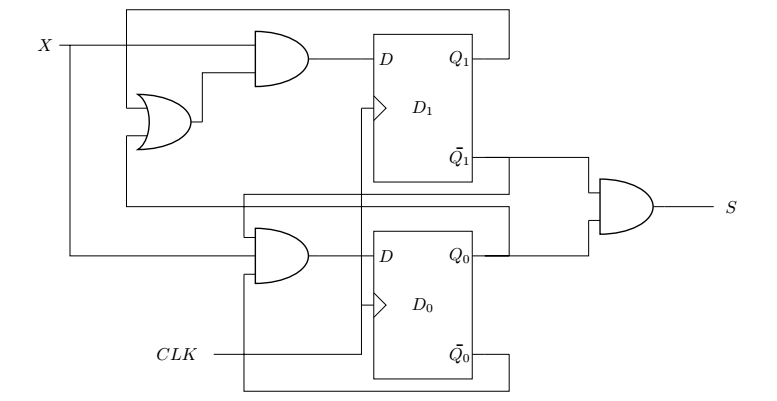
\includegraphics[scale=0.5]{Ejercicio3/Circuitos/LogicaEj3}
\caption{Lógica de entrada}
\end{center}
\label{Logica_de_entrada_Ej3}
\end{figure}

 \begin{figure}[H]
\begin{center}
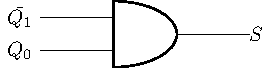
\includegraphics[scale=0.75]{Ejercicio3/Circuitos/SalidaEj3}
\caption{Lógica de salida}
\end{center}
\label{Logica_de_salida_Ej3}
\end{figure}